\documentclass[a4j,12pt]{jreport}
%\documentclass{jreport}
\usepackage[dvipdfmx]{graphicx}
% \usepackage[dvipdfmx]{graphics}
\usepackage{amsmath,amssymb}
% \usepackage{amsmath}
%\usepackage{pxjahyper}
\usepackage{here}
\usepackage{algorithm}
\usepackage{algorithmic}
%\usepackage{algpseudocode}
\usepackage{hhline} 
\usepackage[hang,small,bf]{caption}
\usepackage[subrefformat=parens]{subcaption}
\usepackage{url}
\usepackage{bm}
\captionsetup{compatibility=false}
 

\def\syaji{ \chapter*{謝辞} \addcontentsline{toc}{chapter}{謝辞}}
\renewcommand{\bibname}{参考文献}
\setlength{\textheight}{\paperheight}
\setlength{\topmargin}{4.6mm}
\addtolength{\topmargin}{-\headheight}
\addtolength{\topmargin}{-\headsep}
\addtolength{\topmargin}{-\headheight}
\addtolength{\textheight}{-60mm}

\setlength{\textwidth}{\paperwidth}
\setlength{\oddsidemargin}{-0.4mm}
\setlength{\evensidemargin}{-0.4mm}
\addtolength{\textwidth}{-50mm}

\begin{document}

%%%%%%%%%%%%%%%%%%%%%
% 表紙
%%%%%%%%%%%%%%%%%%%%%
\thispagestyle{empty}
\begin{center}
\begin{Large}
\vspace*{0.7cm}
{\large 中央大学大学院理工学研究科情報工学専攻\\修士論文}\\
\vspace*{2.5cm}
{\LARGE\bf 煙シミュレーションのための部分空間法の高速化}\\
\vspace*{0.7cm}
{\sf Accelerated Subspace Method for 3D Smoke Simulation}\\
\vspace*{6.5cm}
須之内 俊樹\\
Toshiki SUNOUCHI\\
学籍番号\hspace*{1zw}23N8100018B\\
\vspace*{2.5cm}
指導教員\hspace*{1zw} 森口 昌樹 准教授\\
\vspace*{2.5cm}
2025年3月\\
\end{Large}
\end{center}


%%%%%%%%%%%%%%%%%%%%%
% 概要
%%%%%%%%%%%%%%%%%%%%%
\newpage
\renewcommand{\baselinestretch}{1.25} \selectfont
\pagenumbering{roman}


\begin{center} {\large \bf{概 要}} \end{center}

\vspace{1zw} \noindent
{\bf キーワード: }流体シミュレーション,部分空間法,Snapshot 固有直交分解,Cubature

%%%%%%%%%%%%%%%%%%%%%
% 目次
%%%%%%%%%%%%%%%%%%%%%
\tableofcontents


\newpage
\pagenumbering{arabic}

%%%%%%%%%%%%%%%%%%%%%
% 1章
%%%%%%%%%%%%%%%%%%%%%
\chapter{序論} \label{chapter:1}

流体シミュレーションとは,コンピュータを用いて,流体の位置,速度,圧力などの物理量を計算するものである.表現できる流体は,空気,ガスなどの気体や,水,土砂の混ざった水,蜂蜜のような粘性がある液体,砂粒などの固体の粒など多岐にわたる.また,2次元と3次元を扱うことができる.2次元では,水面に広がる波紋や,異なる流体が作り出すマーブル模様などがシミュレーションでき,3次元では私たちの身の回りの現象を広くシミュレーションすることができる.計算した結果を人間が見やすいように可視化することで,流体力学の理論だけでは把握することが困難な,空間に広がる流体の物理量の分布を把握することができるようになる.

流体シミュレーションは,工学分野とコンピュータグラフィックの分野で活用されている.工学分野では,流体に触れる製品の設計・開発において,製品と流体の相互関係を事前にシミュレーションすることで,実験のコスト削減などに役立っている.コンピュータグラフィックスの分野では,水や煙のそれらしいアニメーションを生成し,映像作品やゲームの演出に役立っている.コンピュータグラフィックスの分野では,現実の物理現象に忠実な計算よりも,それらしい振る舞いを高速に計算することや,ユーザーが表現を操作しやすいことが重要視されている.

近代的な高解像度の流体表現は計算負荷が高く,高速化の研究が盛んに行われている.コンピュータグラフィックスの分野における高速化において,大規模並列計算手法の適用性が重要視されている.流体シミュレーションの計算はGPUによる高速化と相性が良く,高速化手法もGPUに適用できるものが望まれている.
また,前処理によってシミュレーション計算に利用する行列の次元を削減し計算負荷を削減する,部分空間法が存在する.これらの手法はシミュレーション計算は高速に行うことができるが,前処理の計算負荷や空間計算量が大きいことに注意が必要である.

本研究では,部分空間法の計算負荷削減により,前処理にかかる時間の短縮を目指す.
	%\section{流体シミュレーションの活用}
	%\section{流体シミュレーションの課題}
	%\section{流体シミュレーションの高速化手法}
	%	\subsection{大規模並列計算}
	%	\subsection{部分空間法を用いた次元削減}
	%\section{本研究の目的}
%%%%%%%%%%%%%%%%%%%%%
% 2章
%%%%%%%%%%%%%%%%%%%%%
\chapter{関連研究} \label{chapter:2}
	%\section{ナビエ・ストークス方程式}
	%\section{計算手法}
	\section{流体シミュレーション}\label{sec:fractional}
		%\subsection{ナビエ・ストークス方程式}
		%\subsection{離散化手法}
		%\subsection{Semi-Lagragian法を用いた移流項計算}
		%\subsection{Corinの射影法を用いた圧力項計算}
		まず,流体シミュレーションの分野で一般的に使われている表記の説明をする.位置$\bm{x}$や時刻$t$を指定した物理量を表現する際は,$\bm{u}(\bm{x},t)$のように表記する.
		\begin{quote}
		\begin{itemize}
		%\item $\bm{x}:$ 流体の位置を表すベクトル.シミュレーションする空間によって2次元,または3次元になる.
		%\item $t:$ 時刻を表す変数.シミュレーション開始の時刻を$0$とする.
		\item $\varDelta x,\varDelta t:$ 離散化する計算格子の格子幅,次の時刻までの時間幅.
		\item $\bm{u}$:シミュレーション空間全体の流体の速度ベクトル.$\bm{u}(\bm{x},t)$は三次元ベクトルとなる.
		\item $\bm{p}$:流体の圧力.
		%\item $\bm{u} (\bm{x},t) :$ 位置$\bm{x}$,時刻$t$でのは,
		%\item $p (\bm{x},t) :$ 位置$\bm{x}$,時刻$t$での流体の圧力値.
		\item $\rho,\nu:$ それぞれ,流体の密度,流体の粘性.ここでは位置や時刻によらない定数とする.
		\item $\bm{f}:$ 位置$\bm{x}$,時刻$t$での流体にかかる外力ベクトル.重力などはここに含める.シミュレーションの手法によっては外力を位置$\bm{x}$,時刻$t$によって変化する外力を扱うことができるが,今回は簡単のため,重力のみを扱い,どの位置でも,どの時刻でも一定の値として考える.
		\item $\nabla:$ 空間微分演算子ナブラ.スカラー場に作用させると勾配を表し,ベクトル場に作用させると発散を表す.3次元空間なので,$\nabla=  (\frac{\partial}{\partial x},\frac{\partial}{\partial y},\frac{\partial}{\partial z}) $ 
		\item $\frac{\rm{D}}{\rm{D}t} =\frac{\partial}{\partial t} + \bm{u} (\bm{x},t)  \boldsymbol{\cdot}\nabla$ :
		ラグランジュ微分,または物質微分.流体力学のような,連続体を扱う力学で用いられており,流れに沿って移動する物体と同じように移動する観測者から見た,物理量の時間変化率を表している.
	\end{itemize}
	\end{quote}
	下記の式\ref{eq:Navie}で表される式を,ナビエ・ストークス方程式とよび,これは流体力学の支配方程式である.非線形二階微分方程式となっており,代数的に一般解を求める事ができない.
	下記の式\ref{eq:compressed}は流体の連続の式と呼ばれる,質量保存や流量保存を表す式である.水や砂粒のように圧縮されない流体を扱うときは,流体の密度が常に一定,つまり密度の時間微分が0になり,それに伴い式\ref{eq:compressed}の左辺の第二項も0になる.これにより,式\ref{eq:uncompressed1}と,式 \ref{eq:uncompressed} を得る.式 \ref{eq:Navie} と式\ref{eq:uncompressed} または式 \ref{eq:uncompressed1}を連立することで非圧縮性流体の速度を求めることができる.ナビエ・ストークス方程式を扱う際は,コンピューターで近似解を解析的に求める手法が用いられる.
	
	\begin{equation}\label{eq:Navie}
		\frac{\partial}{\partial t}\bm{u} (t)  = - (\bm{u} (t)  \boldsymbol{\cdot}\nabla) \bm{u} (t)   - \frac{1}{\rho}\nabla \bm{p} (t)  + \nu\nabla^2\bm{u} (t)  + \bm{f}
	\end{equation}
	\begin{equation}\label{eq:compressed}
		\frac{\rm{D}}{\rm{Dt}}\rho + \nabla\boldsymbol{\cdot}\bm{u} (t)  = 0
	\end{equation}
	\begin{equation}\label{eq:uncompressed1}
		\frac{\rm{D}}{\rm{Dt}}\rho  = 0
	\end{equation}
	\begin{equation}\label{eq:uncompressed}
		\nabla\boldsymbol{\cdot}\bm{u} (t)  = 0
	\end{equation}

%移流項は非線形であり,その他は線形である.
一般の非線形微分方程式は厳密な解析的解法が存在せず,様々な条件を設定した上で,数値解法により離散化し,近似解を求めるのが一般的である.ナビエ・ストークス方程式の数値解法は,分離解法と連成解法が存在する.分離解法は微分方程式の各項ごとに計算を分割する手法であり,線形問題の収束性が良い利点がある一方,分割した項同士の相互作用を計算できないため,厳密な現象の再現が困難であるという欠点がある.特に圧力の計算を分離するMarker And Cell法 (MAC法) \cite{MAC}と呼ばれる手法をLosassoらが提案し,MAC法は現在では圧力を分離する解法のことを広く指す.全ての項を個別に分割して解く手法としてフラクショナルステップ法が存在する.式 \ref{eq:Navie} の右辺の第一項を移流項,第二項を圧力項,第三項を粘性項,第四項を外力項と呼ぶ.連成解法は分離せずに解くため,より正確に現象の再現ができる一方.計算負荷が高いことや収束性が悪いという欠点がある.分割法はコンピュータグラフィックスや流体解析の分野で広く用いられており,扱う手法によって詳細に計算したい相互作用を選択する.

以降はフラクショナルステップ法によるナビエ・ストークス方程式の分割方法を説明する.まず,上記の式\ref{eq:Navie}の時間微分に前進差分を適用し,以下を得る.
\[
\bm{u} (t + \varDelta t) =   \bm{u} (t)-\varDelta t (\bm{u} (t)  \boldsymbol{\cdot}\nabla) \bm{u} (t)- \frac{1}{\rho}\nabla \bm{p}  (t)  + \nu\nabla^2\bm{u} (t)  + \bm{f}) 
\]

この式を,中間子$\bm{u_0}$から$\bm{u_3}$を用いて,以下のように各項ごとに分割して計算する.
\begin{equation}\label{eq:force}
	\bm{u_0} =  \bm{u} (t)  - \varDelta t \bm{f} 
\end{equation} 
\begin{equation}\label{eq:advect}
	\bm{u_1} (\bm{x}) = \bm{u_0} (\bm{x}) - \varDelta t (\bm{u_0}(\bm{x})  \boldsymbol{\cdot}\nabla) \bm{u_0}(\bm{x})
	%\bm{u_1}(\bm{x}) = \bm{u_0}(\bm{x}  - \varDelta t \bm{u_0})
\end{equation}
\begin{equation}\label{eq:diffusion}
	\bm{u_2}   =  \bm{u_1} - \varDelta t \nu\nabla^2\bm{u_1}
\end{equation}
\begin{equation}\label{eq:pressure}
	\bm{u} (t + \varDelta t)= \bm{u_3}  =  \bm{u_2} - \varDelta t \frac{1}{\rho}\nabla \bm{p} 
\end{equation} 

ここで,式\ref{eq:force}は外力項,式\ref{eq:advect}は移流項,式\ref{eq:diffusion}は粘性項,式\ref{eq:diffusion}は粘性項,式\ref{eq:pressure}は圧力項を計算する式である.

%Losassoらが提案したMarker And Cell法 (MAC法) \cite{MAC}と呼ばれる手法は,時間微分の離散化に前進差分を用いてナビエストークス方程式の数値解を求める代表的な手法である.MAC法は仮の速度$\bm{u}^*$を用いて以下のようにナビエ・ストークス方程式を分割し,それぞれ個別に計算を行う.ここで,時刻の偏微分に前進差分$\frac{\partial}{\partial t}\bm{u} (\bm{x},t) = \frac{\bm{u} (\bm{x},t + \varDelta t)- \bm{u} (\bm{x},t )}{\varDelta t}$を用いている.
%\begin{equation}
%	\bm{u} (\bm{x},t + \varDelta t)  =  \bm{u}^* - \varDelta t (\frac{1}{\rho}\nabla p (\bm{x},t)  + \nu\nabla^2\bm{u} (\bm{x},t)  + \bm{f}) 
%\end{equation} 

%\begin{equation}
%	\bm{u}^* = \bm{u} (\bm{x},t)  - \varDelta t (\bm{u} (\bm{x},t)  \boldsymbol{\cdot}\nabla) \bm{u} (\bm{x},t)  
%\end{equation}

ナビエストークス方程式の空間の離散化については,大きく分けて格子法(Eulerian)と粒子法(Lagrangian)がある.
格子法とは,流体を扱う空間を正方形や立方体の格子に区切り,格子の中心や辺,頂点などに物理量を配置して計算する方法である.区切る格子の数が多いほど,流体の詳細な動きが計算できるが,計算負荷は増加する.格子法の利点は,規則正しく並んだ格子で空間を離散化することで,微分演算を差分法などの方法で近似することができることや,境界条件の設定が容易であることが挙げられる.一方で,格子法の欠点は,格子の大きさよりも細かい表現が正確に行えないことや,格子内の流体の粒子の運動を平均化することにより,個々の粒子の詳細な運動を追跡することができないことが挙げられる.これらの欠点により,薄く広がった流体の運動や,水飛沫などを表現することが困難である.

粒子法は,流体の粒子の運動を追跡する手法であり,薄く広がった流体の運動や水飛沫などを表現することが容易である利点がある一方で,計算精度の保証が不十分であることや,境界条件の設定が煩雑になるという欠点がある.

格子法と粒子法は固体にも適用することが可能であり,流体とは異なる支配方程式を用いて変形や移動を計算することができる.流体と固体の相互関係をシミュレーションする際は,格子法と粒子法をそれぞれ個別に適用することが可能である.また,流体の移流項のみを粒子法を用いて計算し,そのほかを格子法で計算するなど,各項の計算について個別に適用する手法が存在する.
%微分計算の差分近似によって,無視されてしまう項が存在する.格子法での移流項の計算に用いられる差分近似で無視される項を,数値拡散,または人工粘性と呼ぶ.格子法での移流項の計算には風上差分がよく用いられるが,簡単のため,前進差分を用いる.格子法の欠点は,この数値拡散が決して小さくないため,移流項の精度があまりよくないことである.しかし,以下の移流項の計算によって,移流項の数値拡散として粘性項に似た形の式が現れる.従って,粘性項は移流項の数値拡散として扱い,まとめて計算されることが多い.また,水飛沫などの,液体が細かく分散するような計算は困難である.これは,微分の計算を差分で近似することで,隣接する格子との相互関係を用いて計算することになるため,液体が分散すると計算がうまくいかないためである.


\section{部分空間法}\label{sec:Subspace}
部分空間法は,ベクトル空間をより低次元の部分空間に射影し,数値シミュレーションにおける計算負荷を軽減する手法である.流体シミュレーションにおける部分空間法は,モデル縮約やモデル縮退とも呼ばれている.扱うベクトルデータやシミュレーションの計算を低次元の部分空間に射影して行い計算負荷を軽減する.以下では,部分空間法の理論の概要を説明する.

\subsection{部分空間への射影}
シミュレーションの前処理として,$n$次元ベクトル$\bm{x}$を$r$次元ベクトル$\bm{\tilde{x}} $に変換する,$n \times r$直交行列$\mathbf{A}$を考える.以下の2式が成り立つ.
 	\[
 		\bm{\tilde{x}}  = \mathbf{A^T}\bm{x}
 	\]
	\[
		\bm{x} = \mathbf{A}\bm{\tilde{x}} 
	\]	
	また,$\bm{\tilde{x'}}  = \mathbf{A^T}\bm{x'}$を満たす$n$次元ベクトル$\bm{x'}$,$r$次元ベクトル$\bm{\tilde{x'}} $について,以下の2式が成り立つような,任意の$m \times n$行列$\mathbf{F}$,任意の$m \times r$行列$\mathbf{\tilde{F}}$を考える.
	\[
		\bm{x'} = \mathbf{F}\bm{x}
	\]
	\[
		\bm{\tilde{x'}}  = \mathbf{\tilde{F}}\bm{\tilde{x}} 
	\]
$\bm{\tilde{x'}}  = \mathbf{A^T}\bm{x'}$に,$\bm{x'} = \mathbf{F}\bm{x}$と,$\bm{x} = \mathbf{A}\bm{\tilde{x}} $を代入することで,
	\[
		\bm{\tilde{x'}}  = (\mathbf{A^T}\mathbf{F}\mathbf{A})\bm{\tilde{x}} 
	\]
	が得られる.$\bm{\tilde{x'}}  = \mathbf{\tilde{F}}\bm{\tilde{x}} $と比較すると,
	\[
	\mathbf{\tilde{F}} = \mathbf{A^T}\mathbf{F}\mathbf{A}
	\]
	が得られる.
	
以上により,任意のベクトルに対する行列積を,$n \times r$直交行列$\mathbf{A}$を用いて部分空間に射影することができる.

\subsection{Snapshot固有直交分解}
流体シミュレーションにおいて,部分空間に射影したベクトルを用いてシミュレーション計算をするためには,射影後のベクトルも流体の非圧縮性条件等の性質を満たさなければならない.そのような射影を達成する行列$\mathbf{A}$を得る手法として,Snapshot固有直交分解がある.行列$\mathbf{A}$を既存の流体のデータを主成分分析を用いて計算することで,流体の性質を満たした射影が可能である.
以降はSnapshot固有直交分解の具体的な計算方法について説明する.
	
	時刻$t \{t \in N, 0 \le t \le m\}$の$n$次元ベクトルデータ$\bm{u_t}$を用いて,$n\times m$行列$\mathbf{S}$を定義する.
		 \[ \mathbf{S} = 
        		\begin{bmatrix}
   | & | &  & |\\
   \bm{u}_0 & \bm{u}_1 &\cdots  & \bm{u}_{m-1} \\
   | & | &  & |
\end{bmatrix}
\]
次に,行列$\mathbf{S}$主成分分析を行うため,$n \times r$行列$\mathbf{A}$について以下の最小化問題を考える.ここで$r$は抽出したい主成分の数である.
\[
min || \mathbf{S} -  \mathbf{A}\mathbf{A^T} \mathbf{S}||^2_F
\]


この最小化問題の解となる行列$\mathbf{A}$は,$\mathbf{S}\mathbf{S^T}$の固有ベクトル$\bm{v_i}(0 \le i \le r-1)$を用いて,以下の行列になる.
 \[ 
 \mathbf{A}  = 
        		\begin{bmatrix}
   | & | &  & |\\
   \bm{v}_0 & \bm{v}_1 &\cdots  & \bm{v}_{r-1} \\
   | & | &  & |
\end{bmatrix}
\]
ここで,固有ベクトル$\bm{v_i}$に対応する固有値を$\lambda_i$は,$\lambda_0 \ge \lambda_1 \cdots \ge \lambda_i \ge \lambda_{n-1} $を満たすとする.$\mathbf{S}\mathbf{S^T}$は対称行列になっているため,固有ベクトルは互いに直交し,$\mathbf{A^{-1}} = \mathbf{A^T}$となる.%また,$n \times n$行列$\mathbf{S^T}\mathbf{S}$ と$m\times m$行列$\mathbf{S}\mathbf{S^T}$の固有ベクトルは

次に,行列$\mathbf{A}$を用いて$\bm{u}$を$\bm{\tilde{u}}$に射影するとき,$\bm{\tilde{u}}$が流体の非圧縮性条件$\nabla\boldsymbol{\cdot}\bm{\tilde{u}} = 0$を満たしていることを確かめる.行列$\mathbf{S}$の各列ベクトル$\bm{u_i}$は既存のシミュレーションの速度データであるため,流体の非圧縮性条件$\nabla\boldsymbol{\cdot}\bm{u_i} = 0$を満たす.このことから,
\[
	\nabla\boldsymbol{\cdot}\mathbf{S}\ = \sum_{0 \le i \le n-1}\nabla\boldsymbol{\cdot}\bm{u_i} = 0
\]
が成り立つ.

また,行列$\mathbf{S}\mathbf{S^T}$の固有ベクトル$\bm{v_i}$と,それに対応する固有値を$\lambda_i$とすると,固有値と固有ベクトルの定義から以下が成り立つ.
\[
	\mathbf{S}\mathbf{S^T}\bm{v_i} = \lambda_i\bm{v_i}
\]
両辺に左から$\nabla\boldsymbol{\cdot}$を取ることにより,
\[
	(\nabla\boldsymbol{\cdot}\mathbf{S})\mathbf{S^T}\bm{v_i} = \lambda_i\nabla\boldsymbol{\cdot}\bm{v_i}
\]
$\nabla\boldsymbol{\cdot}\mathbf{S}\ = 0$より,0でない$ \lambda_i$について,$\nabla\boldsymbol{\cdot}\bm{v_i} = 0$が成り立つことがわかる.

$n \times n$行列$\mathbf{S}\mathbf{S^T}$の主成分分析を行う代わりに,$\mathbf{S^T}\mathbf{S}$の主成分分析を行い,$\mathbf{S}\mathbf{S^T}$の固有値固有ベクトルを求めることができる.$\mathbf{S}\mathbf{S^T}\bm{v_i} = \lambda_i\bm{v_i}$の両辺に左から$\mathbf{S^T}$をかけることにより,
\[
	(\mathbf{S^T}\mathbf{S})\mathbf{S^T}\bm{v_i} = \lambda_i\mathbf{S^T}\bm{v_i}
\]
を得る.行列$\mathbf{S^T}\mathbf{S}$の固有値は,$\mathbf{S}\mathbf{S^T}$の固有値と一致し,固有値$\lambda_i$対応する固有ベクトル$\bm{u_i}$について,$\bm{u_i} = \mathbf{S^T}\bm{v_i}$であることがわかる.よって,$\mathbf{S^T}\mathbf{S}$の主成分分析により得られた固有ベクトルと$\mathbf{S^T}$の逆行列を用いて,$\mathbf{S}\mathbf{S^T}$の主成分分析を行うことができる.

\subsection{特異値分解を用いる方法}
$n \times r$行列$\mathbf{S}$の特異値分解は,以下のように定義される.
\[
\mathbf{S} = \mathbf{U} \mathbf{\Sigma} \mathbf{V}^T
\]

ここで,\( \mathbf{U} \) は \( n \times n \) のユニタリ行列であり,左特異ベクトルを列ベクトルとして持つ.\( \mathbf{V} \) は \( r \times r \) のユニタリ行列であり,右特異ベクトルを列ベクトルとして持つ.\(\mathbf{ \Sigma }\) は \( n \times r \) の対角行列であり,対角成分には特異値 \( \sigma_1, \sigma_2, \dots, \sigma_r \) が非負の降順で並ぶ.

以下に示す,行列$\mathbf{S^T}\mathbf{S}$の固有値や固有ベクトルと行列$\mathbf{S}$の特異値分解の関係により,$\mathbf{S}\mathbf{S^T}$の主成分分析を行う代わりに,行列\(\mathbf{S}\)の特異値分解を用いることができる.

行列$\mathbf{S^T}\mathbf{S}$の対角化を,以下のように表す.
\begin{equation}\label{eq:diagonalization}
	\mathbf{S^T}\mathbf{S} = \mathbf{P}\mathbf{A}\mathbf{P^{-1}}
\end{equation}
ここで,\(\mathbf{A}\)は\( n \times n \) の対角行列であり,対角成分には行列$\mathbf{S^T}\mathbf{S}$の固有値が降順に並ぶ.\(\mathbf{P}\)の\(i\)列は固有値\(\mathbf{A_{i,i}}\)に対応する固有ベクトルである.

行列\(\mathbf{S}\)の特異値分解より,以下が成り立つ.
\[
\mathbf{S^T}\mathbf{S} = (\mathbf{V} \mathbf{\Sigma} \mathbf{U}^T)(\mathbf{U} \mathbf{\Sigma} \mathbf{V}^T)
\]

行列\(\mathbf{U}\)はユニタリ行列,\(\mathbf{\Sigma}\)は対角行列であるから,
\[
\mathbf{S^T}\mathbf{S} = \mathbf{V}\mathbf{\Sigma^2} \mathbf{V}^T
\]
式\ref{eq:diagonalization}と右辺を比較することによって,\(\mathbf{P} = \mathbf{V} \),\(\mathbf{A} = \mathbf{\Sigma^2} \)であることがわかる.

\subsection{非線形項の計算}
非線形項については,Cubature法を用いた積分計算の計算量削減手法を用いて次元削減を行う.非線形関数$\mathcal{F}$について,$\bm{f} = \mathcal{F}(\bm{x})$とする.ここで,$\bm{f}$,$(\bm{x})$は$n$次元ベクトルである.削減前の$\bm{f}$は,$\mathcal{F}$をシミュレーション空間$\Omega$の全ての計算点$\bm{x_p}$において積分することで求められる.
\[
	\bm{f} = \int_\Omega\mathcal{F}_p(\bm{x_p})
\]
この積分計算をCubature法を用いて次元削減する.
Cubature法はシミュレーション空間全域から適切に計算点を有限個サンプリングし,重み付き和をとることで積分計算を離散化する.
サンプリングした点集合を$P$,サンプリング点$p$に対応する重みを$w_p$とすると,Cubature法は以下のように表せる.
\[
	\bm{f} = \sum_{p=1}^Pw_p\mathcal{F}_p(\bm{x_p})
\]
この式は速度に関する基底を用いて以下のように部分空間へ射影することが可能である.
\[
	\mathbf{U_1}\bm{f} = \sum_{p=1}^Pw_p(\mathbf{U^p_1})^T\mathcal{F}_p(\mathbf{U^p_0}\bm{x})
\]
ここで,$\mathbf{U^p}$は$3 \times n$基底行列$\mathbf{U}$のサンプリング点$p$に関する行を抜粋して作成した,$3 \times r$行列である.$\bm{\tilde{f}}_p$ = $(\mathbf{U^p_1})^T\mathcal{F}_p(\bm{\tilde{u_1}})$とすると,最終的な部分空間に射影した移流項計算は,以下のようになる.
\[
	\bm{\tilde{u_2}} = \sum_{p=1}^Pw_p\bm{\tilde{f}}_p =   \sum_{p=1}^Pw_p(\mathbf{U^p_1})^T\mathcal{F}_p(\bm{\tilde{u_1}})
\]

以降はサンプリング点と重みを評価する手法について説明する.
\begin{equation}
	 \begin{bmatrix}
	 \bm{\tilde{f}}^0_0	&\cdots	&\bm{\tilde{f}}^p_0	&\cdots	&\bm{\tilde{f}}^P_0\\
		\vdots		&\ddots		&\vdots		&		&\vdots			\\
	\bm{\tilde{f}}^0_t	&\cdots	&\bm{\tilde{f}}^p_t	&\cdots	&\bm{\tilde{f}}^P_t\\
		\vdots		&		&\vdots			&\ddots		&\vdots			\\
	\bm{\tilde{f}}^0_T	&\cdots	&\bm{\tilde{f}}^p_T	&\cdots	&\bm{\tilde{f}}^P_T\\
	\end{bmatrix}
	\begin{bmatrix}
	w_0 	\\
	\vdots \\
	w_p \\
	\vdots \\
	w_P
	\end{bmatrix}=
	\begin{bmatrix}
	\bm{\tilde{f}}_0 	\\
	\vdots \\
	\bm{\tilde{f}}_t \\
	\vdots \\
	\bm{\tilde{f}}_T
	\end{bmatrix}
\end{equation}

ここで,$\bm{\tilde{f}}_t $はシミュレーションのSnapshot行列$\mathbf{S}$から抜粋した$t$番目の速度$\bm{u}_t$を用いて$\bm{\tilde{f}}_t = \mathbf{U}_1\bm{u}_t$とする.$\bm{\tilde{f}}^p_t$はサンプリング点に関する値$\mathbf{U^p}_1\bm{u^p}_t$である.
%$\mathbf{A}$を用いて$\bm{u}$を$\bm{\tilde{u}}$に射影するとすると,$\bm{\tilde{u}} = \mathbf{A^T}\bm{u}$より,以下が成り立つ.
%\[
%	\bm{\tilde{u}} =  \begin{bmatrix}
%	\bm{v_0}\boldsymbol{\cdot}\bm{u}\\
%	\bm{v_1}\boldsymbol{\cdot}\bm{u}\\
%	\vdots\\
%	\bm{v_r}\boldsymbol{\cdot}\bm{u}
%\end{bmatrix}
%\]
	%\subsection{}
	%\section{ボリュームデータの可視化手法}
\chapter{煙の流体シミュレーション}
流体シミュレーションを行う際,境界条件や外力項を適切に設定することで流体の振る舞いを操作することができる.この章では文献\cite{fedkiw}を参考に,フラクショナルステップ法を格子法により離散化した煙の流体シミュレーションを実装する方法と,スライスベースのボリュームレンダリングによる可視化手法について説明する.%この手法で得られたシミュレーションデータを用いて部分空間法に用いるSnapshot固有直交分解を行う.

\section{格子法による離散化}
\begin{figure}[H]
\begin{center}
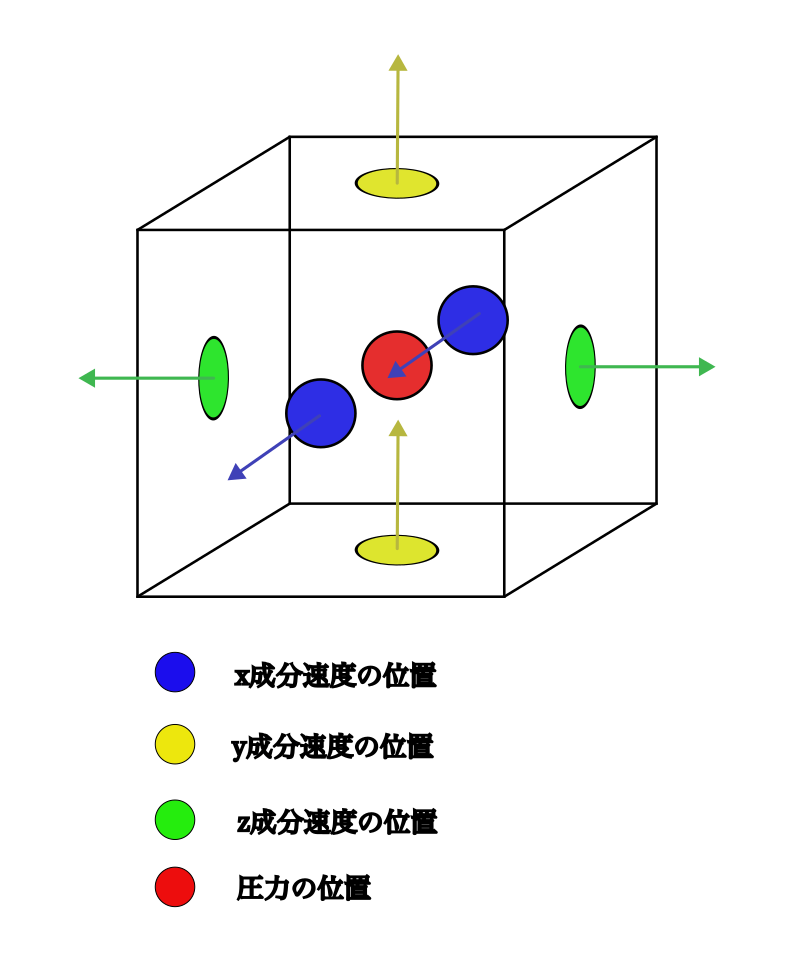
\includegraphics[width=80mm]{images/3dstaggerd.png}
\caption{スタッガード格子}
\label{fig:staggerd}
\end{center}
\end{figure}
格子法による空間の離散化は,扱う格子によって様々な手法が存在する.例えば物理量を格子の中心に配置するコロケート格子や,速度成分を格子の面の中心に配置するスタッガード格子が存在する.コロケート格子は流体の格子の形状によらず適用できるが,境界条件の設定が煩雑である.スタッガード格子は適用が立方体格子などに限定される一方,境界条件の設定が容易である.スタッガード格子は上の図\ref{fig:staggerd}のように,圧力の定義位置を格子の中心とし,格子面の中心にその格子面と垂直な流速の成分の位置を定義する.例えば$xy$平面に並行な格子面には,その地点での流速の$z$成分を配置する.

%\begin{figure}[htbp]


シミュレーション空間の$\rm{x,y,z}$軸方向の分割数を$\rm{nx,ny,nz}$とする.このとき空間解像度は$\rm{nx \cdot ny \cdot nz}$となり,速度の$\rm{x,y,z}$成分の空間解像度はそれぞれ$(nx+1) \cdot ny \cdot nz$,$nx \cdot (ny+1) \cdot nz$,$nx \cdot ny \cdot (nz+1)$となる.本論文では,$nx = ny =nz$とし,速度$\bm{v}$と圧力$\bm{p}$は以下のベクトルに離散化する.
\begin{itemize}
	\item	$\bm{v_x}$:$(nx+1) \times ny \times nz$次元ベクトル.
	\item	$\bm{v_y}$:$nx \times (ny+1) \times nz$次元ベクトル.
	\item	$\bm{v_z}$:$nx \times ny \times (nz+1)$次元ベクトル.
	\item	$\bm{v}$:$3\times(nx+1) \cdot ny \cdot nz $次元ベクトル.
	\item $\bm{p}$:$nx \cdot ny \cdot nz$次元ベクトル.
\end{itemize}
ここで$\bm{v}$の$v_0$から$v_{(nx+1) \cdot ny \cdot nz -1}$には速度の$x$成分,
$v_{(nx+1) \cdot ny \cdot nz }$から$v_{2\times(nx+1) \cdot ny \cdot nz - 1}$には速度の$y$成分,
$v_{2\times(nx+1) \dot ny \cdot nz - 1}$から$v_{3\times(nx+1) \cdot ny \cdot nz - 1}$には速度の$z$成分を保存する.
また,位置$\bm{x} =(i,j,k)$における速度$\bm{v} (\bm{x})$を,以下のように表す.
\[
	\bm{v} (\bm{x})= 
	 \begin{bmatrix}
		\bm{v_x}(i,j,k)\\
		\bm{v_y}(i,j,k)\\
		\bm{v_z}(i,j,k)
	\end{bmatrix}
\]
前進差分を用いた空間の偏微分の離散化の例として,スタッガード格子を用いた以下の偏微分の離散化を上記のベクトルを用いて表現することを考える.
\[
\frac{\partial}{\partial \bm{x}}\bm{u} (\bm{x}) = \frac{\bm{u}(\bm{x}+\varDelta \bm{x})  - \bm{u} (\bm{x}) }{\varDelta \bm{x}}
\]
ここで,$\bm{u} (\bm{x})$は位置$\bm{x}$での速度を表す三次元ベクトルである.
スタッガード格子の一辺の長さを$\varDelta L = \varDelta \bm{x}$,流体の位置ベクトル$\bm{x}$を自然数$i(0 \le i \le nx-1),j(0 \le j \le ny-1),k(0 \le k \le nz-1)を用いて,$$\bm{x} = (i\varDelta L,j\varDelta L,k\varDelta L)$とすると,以下のようになる.
\[
\frac{\bm{u}(\bm{x}+\varDelta \bm{x})  - \bm{u} (\bm{x}) }{\varDelta \bm{x}}
= \begin{bmatrix}
\frac{\bm{v_x}(i+1,j,k)  - \bm{v_x} (i,j,k) }{\varDelta L}\\
\frac{\bm{v_y}(i,j+1,k)  - \bm{v_y} (i,j,k) }{\varDelta L}\\
\frac{\bm{v_z}(i,j,k+1)  - \bm{v_z} (i,j,k) }{\varDelta L}
\end{bmatrix}
\]

\subsection{ディリクレ境界条件}
流体シミュレーションにおいて,流体と流体以外の境界面の物理量の条件を設定する必要がある場面がある.これを境界条件と呼び,文献\cite{fedkiw}では境界における物理量を事前に一定の値に設定するディリクレ境界条件が用いられており,境界における物理量は$0$と設定する.ディリクレ境界条件は速度成分を都度初期化することで適用できるほか,境界成分に対応する成分を0とした単位行列を用いた表現も可能である.ディリクレ境界条件を表現する行列を$\mathbf{D}$とすると,$\mathbf{D}$の$i,j$成分は以下のように定義される.
\begin{equation}
	\mathbf{D}_{i,j} = \begin{cases}
 	1 	& i = j かつ iは境界成分でない\\
 	0  		& その他\\
 \end{cases}
\end{equation}
この行列表現は通常の流体シミュレーションでは不要であるが,部分空間法を用いた流体計算では境界成分に対応する値を変更することが困難なため,境界条件を行列積を用いて表現する手法が用いられている.

\subsection{外力項計算}
外力項では,再現したい現象になるような外力を与えなければならない.コンピュータグラフィックスにおける気体の外力は,気体にかかる重力と,温度差による対流を発生させる力,気体が渦巻くように与える力などをユーザーがパラメータによって調整できるようにする計算方法が一般的である.本実験では重力と,対流を発生させる力を加える.よりそれらしい振る舞いを再現するため,他の計算では定数として扱う密度や温度を,ここでは位置と時刻によって変化するデータとして計算する.
位置$\bm{x}$における気体の密度,温度をそれぞれ$\rho(\bm{x})$,$T(\bm{x})$,環境温度を$T_{amb}(\bm{x})$,重力の方向ベクトルを$\bm{d}$とすると,気体に働く外力は以下のようになる.

\begin{equation}\label{eq:buoyancy}
	\bm{f_{buoy}(\bm{x})} =  \alpha \rho(\bm{x})\bm{d}+ \beta(T(\bm{x})- T_{amb}(\bm{x}))\bm{d}
\end{equation} 
ここで,$\alpha$,$\beta$はユーザーが設定するパラメータであり,それぞれ重力と対流の力を調整する.最終的な外力項計算は以下のようになる.
\begin{equation}
	\bm{u_0} =  \bm{u}  - \varDelta t \bm{f_{buoy}} 
\end{equation} 

%!!!スタッガードグリッドのスキームが速度と外力で異なる話
%\begin{equation}\label{eq:confinent}
%	\bm{f_{conf}(\bm{x})} =  
%\end{equation} 

\subsection{移流項計算}
移流項は流体の物理量が流体の速度場によって移動する様を計算することができる.移流項は非線形方程式であり,様々な計算方法が存在する.文献\cite{fedkiw}のSemi-Lagrangian法を紹介する.Semi-Lagrangian法
は計算負荷が小さく,陰解法により安定した計算結果を得ることができるため,コンピュータグラフィックスの分野で広く用いられている.

%Semi-Lagrangian法は移流計算を物質微分$\frac{\rm{D}}{\rm{D}t} =\frac{\partial}{\partial t} + \bm{u} (\bm{x},t)  \boldsymbol{\cdot}\nabla$を用いて行う.
%簡単のため,ナビエストークス方程式から粘性項と外力項を取り除いた,オイラー方程式と呼ばれるものについて考える.
Semi-Lagrangian法は,格子に配置されている計算点上の物理量を計算する格子法(Eulerian)の特徴と,移動する計算点を追跡し計算を行う粒子法(Lagrangian)の特徴を両方持っている計算手法である.
移流項の計算$$\bm{u_1} = \bm{u_0}  - \varDelta t (\bm{u_0}  \boldsymbol{\cdot}\nabla) \bm{u_0}$$を変形し,時刻の偏微分に対し前進差分$\frac{\partial \bm{u}}{\partial t} = \frac{\bm{u_1} - \bm{u_0}}{ \varDelta t }$すると,以下の式が得られる.
\[
\frac{\partial \bm{u}}{\partial t}   +(\bm{u_0}  \boldsymbol{\cdot}\nabla) \bm{u_0} = 0
\]
この式は以下の輸送方程式と呼ばれる式の特殊な場合であり,輸送方程式は一般の物理量$\phi$に関して適用可能である.
\begin{equation}\label{eq:transfer}
	\frac{\partial {\phi}}{\partial t}  +(\bm{u}  \boldsymbol{\cdot}\nabla) {\phi} = 0
\end{equation} 
この輸送方程式が成り立つとき,位置$\bm{x}$,時刻$t$における物理量$\phi(\bm{x},t)$について,以下の式が成り立つ.
\begin{equation}\label{eq:semi-Lagrangian}
	{\phi}(\bm{x},t) = {\phi}(\bm{x}  - \varDelta t \bm{u},t)
\end{equation} 
Semi-Lagrangian法を以下のように流速に適用することで移流項の計算を行う.また,密度や温度などに対して適用することで,空間の速度ベクトル場に沿って気体が運動する様子を再現することができる.
\begin{equation}\label{eq:advect}
	\bm{u_1}(\bm{x}) = \bm{u_0}(\bm{x}  - \varDelta t \bm{u_0})
\end{equation}
以下では,輸送方程式\ref{eq:transfer}が成り立つとき,式\ref{eq:semi-Lagrangian}が成り立つことを確認する.$\bm{x}$にある物理量は$\bm{u} (\bm{x}) $に沿って$\varDelta t\bm{u} (\bm{x})$移動すると仮定すると,移動前の物理量は$\phi(\bm{x} -  \varDelta t\bm{u} (\bm{x}))$となる.この間の物理量の変化$\varDelta {\phi}$は以下のようになる.
\[
\varDelta \phi = \phi( \bm{u} (\bm{x}),t) - \phi (\bm{x} - \varDelta t\bm{u} (\bm{x}),t)
\]
これを一次のテイラー展開を用いて表すと,
\[
\varDelta \phi   = \frac{\partial \bm{u} (\bm{x}) }{\partial \bm{x}}\phi (\bm{x},t) \varDelta t + \frac{\partial \phi (\bm{x},t) }{\partial t}\varDelta t
\]
$\frac{\partial \bm{u} (\bm{x}) }{\partial \bm{x}}\phi (\bm{x},t)= (\bm{u}(\bm{x}) \boldsymbol{\cdot}\nabla)\phi(\bm{x},t)$より,
\[
 \frac{\varDelta \phi}{\varDelta t} =  (\bm{u}(\bm{x})\boldsymbol{\cdot}\nabla) \phi(\bm{x},t) + \frac{\partial \phi(\bm{x},t) }{\partial t}
 \]
 
 右辺が輸送方程式\ref{eq:transfer}になっていることから,$ \varDelta \phi =0$が成り立つ.
$\varDelta \phi = \phi( \bm{u} (\bm{x})) - \phi (\bm{x} - \varDelta t\bm{u} (\bm{x}))= 0$より,式\ref{eq:semi-Lagrangian}が成り立つことが確認できる.
\subsection{粘性項計算}
粘性項は流体が徐々に周囲に広がっていく様を計算することができる.粘性項計算は$\varDelta t \nu\nabla^2$を行列を用いて表現することで,以下のように行列積を用いて表すことができる.
\begin{equation}\label{eq:discrete Laplacian}
	\bm{u_2}   =  \bm{u_1} - \varDelta t \nu\nabla^2\bm{u_1} = (\mathbf{I} -  \frac{\varDelta t \nu}{(\varDelta x)^2}\mathbf{L})\bm{u_1} = \mathbf{W}\bm{u_1}
\end{equation}
ここで,$\nabla^2$の離散化を行列$\mathbf{L}$を用いて表すことを考える.行列$\mathbf{L}$を$v_0$から$v_{n-1}$の$n$個の頂点を持つ無向グラフに対して離散ラプラシアンと呼び,$n \times n$行列$\mathbf{L}$の成分$\mathbf{L}_{i,j}$は以下のように定義される.ただし,無向グラフは自己ループを持たないとする.
\begin{equation}
	\mathbf{L}_{i,j} = \begin{cases}
 	deg(v_i) 	& i = j\\
 	-1  		& v_iとv_jが接続している\\
 	0  		& その他\\
 \end{cases}
\end{equation}
スタッガード格子を用いた流体シミュレーションにおいて,無向グラフは流体のそれぞれの速度成分ごとの連結成分を持つとする.つまり,本論文のシミュレーションにおいては連結成分数は3であり,それぞれの頂点数は$(nx+1) \times ny \times nz$である.また,シミュレーション境界を除く速度に対応する次数は$6$であり,シミュレーション境界上の成分はディリクレ境界条件によって速度成分が$0$になるため,任意の値でよい.よって粘性項計算を表現する行列$\mathbf{V}$の成分$\mathbf{V}_{i,j}$は以下のように定義される.
 \[
 	\mathbf{V}_{i,j}  = \begin{cases}
 	1 - 6 \frac{\varDelta t \nu}{(\varDelta x)^2} 	& i = j\\
 	 \frac{\varDelta t \nu}{(\varDelta x)^2}  	& v_iとv_jが接続している\\
 	0  				& その他\\
	 \end{cases}
\]

\subsection{圧力項計算}
圧力項計算は,流体の非圧縮性を満たすために流体に圧力勾配による外力を与える計算である.以下では,代表的な圧力項計算手法である,コリンの射影法を紹介する.圧力項計算によって離散化するのは以下の方程式である.
\[
	\bm{u} (t + \varDelta t)=  \bm{u_2} - \varDelta t \frac{1}{\rho}\nabla p
\]
上記の式の両辺の発散をとると,
\[
	\nabla\boldsymbol{\cdot}\bm{u} (t + \varDelta t)=  \nabla\boldsymbol{\cdot}\bm{u_2} - \varDelta t \frac{1}{\rho}\nabla^2 p
\]
が得られる.流体の非圧縮性条件,$\nabla\boldsymbol{\cdot}\bm{u} (t + \varDelta t)= 0$により,左辺は0になるため,
\begin{equation}
\nabla\boldsymbol{\cdot}\bm{u_2} = \frac{\varDelta t}{\rho}\nabla^2 p
\end{equation} 
が得られる.この式を圧力に関するポアソン方程式として解き,$\bm{u} (t + \varDelta t)=  \bm{u_2} - \varDelta t \frac{1}{\rho}\nabla p$に代入することで圧力項計算が完了する.ポアソンの境界条件にはディリクレ境界条件を適用する.

スタッガード格子では圧力と流速の配置されている位置が異なるため,空間微分に対して同じ差分は適応できない.そこで両辺をセルの領域で積分することを考える.
\[
\int_V\nabla\boldsymbol{\cdot}\bm{u_2} dV= \int_V\frac{\varDelta t}{\rho}\nabla^2 \bm{p}  dV
\]
両辺にガウスの発散定理を適用すると,周回積分の形で表せる.
\[
\oint_V\bm{u_2}\boldsymbol{\cdot}\bm{n} dV= \oint_V\frac{\varDelta t}{\rho}\nabla \bm{p}  \boldsymbol{\cdot}\bm{n}dV
\]
左辺から空間微分が消去できたため,右辺の空間微分に対して適切な微分スキームを適用することで,周回積分を離散化することができる.
ここで離散化のため,$x軸方向にi番目,y軸方向にj番目,z軸方向にk番目の格子を$$g_{i,j,k}$,圧力を$p_{i,j,k}$と定義し,図\ref{fig:pressure_model}のようなモデルを考える.

まず,整数$n=0,1,2,\cdots 5$までを,それぞれ格子の各面の方向に割り振る.図\ref{fig:pressure_model}の場合,$n=0$は$x$軸正の方向,$n=1$は$y$軸正の方向,$n=2$は$x$軸負の方向,$n=3$は$y$軸負の方向,$n=4$は$z$軸正の方向,$n=5$は$z$軸負の方向に割り振る.ここで,この整数$n$を用いて,以下の配列や変数を定義する.
\begin{quote}
	\begin{itemize}
		\item $F_n$ 格子の面の各方向に隣接しているものが流体なら$1$,壁面なら$0$を取るブーリアン値.
		
		図\ref{fig:pressure_model}の場合,$n=0$に対応する$x$軸正の方向と,$n=5$に対応する$z$軸負の方向は壁に隣接していて格子がないため,$F_0,F_5 = 0,F_1,F_2,F_3,F_4 = 1$となる.
		\item $D_n$ 格子の面の各方向に垂直で,格子の外側を向く単位ベクトルを表す係数.向いている方向が座標軸の正の向きなら+1,					負の向きなら$-1$を取る整数値.
		
		図\ref{fig:pressure_model}の場合,座標軸の正の方向に向いているのは$n=0,n=1,n=4$に対応する方向で,それ以外は負の方向に向いているため,
		$F_0,F_1,F_4 = 1,F_2,F_3,F_4 = -1$となる.
		\item $p_n$ 割り振られた方向に隣り合っている格子の圧力値.
		図\ref{fig:pressure_model}の場合,$p_0 = p_{i+1,j,k}$,$p_1 = p_{i,j+1,k}$,$p_2 = p_{i-1,j,k}$,$p_3 = p_{i,j-1,k}$,$p_4 = p_{i,j,k+1}$,$p_5 = p_{i,j,k-1}$となるが,境界条件を考えると,壁に隣接している格子との圧力値の勾配を$0$にするため,$p_0 = p_{i,j,k}$,$p_5 = p_{i,j,k}$である.
		\item $\nabla p_n$ 割り振られた方向の圧力勾配.前方差分によって,$\nabla p_n (\bm{x},t)  = \frac{p_n - p_{i,j,k}}{\varDelta x}$と近似できる.
		\item $u_n$ $g_{i,j,k}$において,割り振られた方向の格子面に配置されている流速値.壁に隣接している方向は流速を$0$にするため,$u_0 = 0$,$u_5 = 0$である.
	\end{itemize}
\end{quote}
%\begin{figure}[htbp]
\begin{figure}[H]
\begin{center}
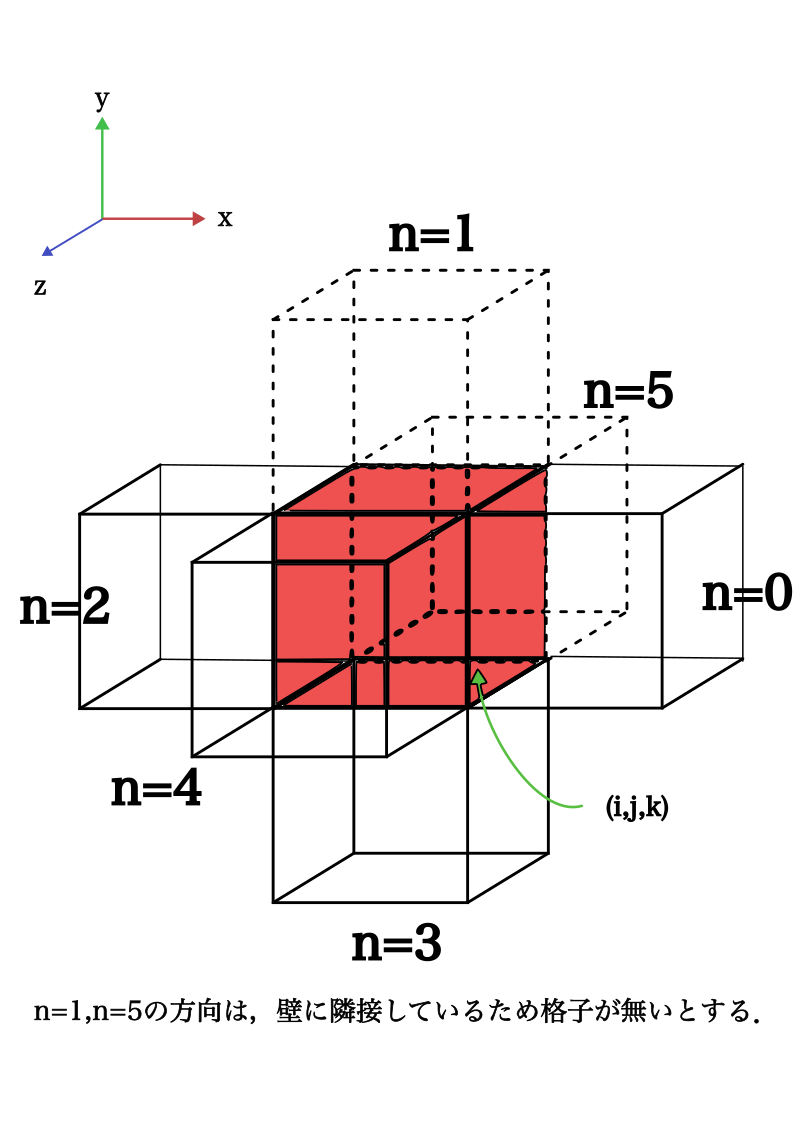
\includegraphics[width=80mm]{images/pressure_model.png}
\caption{圧力計算のモデル}
\label{fig:pressure_model}
\end{center}
\end{figure}
定義した配列や変数を用いて,周回積分の形で表された式を離散化することで,下記の式を得る.
\[
	\sum_{n}\frac{\varDelta t}{\rho}\nabla p_n (\bm{x},t) F_n =  \sum_{n}u_nD_nF_n
\]


%が得られ,圧力勾配を$\nabla p_n (\bm{x},t)  = \frac{p_n - p_{i,j,k}}{\varDelta x}$で近似すると,

%\[
%\sum_{n}\frac{\varDelta t}{\rho}\frac{p_n (\bm{x},t) - p_{i,j,k} (\bm{x},t) }{\varDelta \bm{x}}F_n\varDelta x =  \sum_{n}\bm{u_n}^*D_nF_n\varDelta x
 %\]
%が得られる.この式を整理すると,
%\begin{equation}\label{eq:discretized_pressure}
%\sum_{n}\frac{\varDelta t}{\rho}\frac{p_n (\bm{x},t)  - p_{i,j,k} (\bm{x},t) }{\varDelta \bm{x}}F_n = \sum_{n}\bm{u_n}^*D_nF_n
%\end{equation} 
%が得られる.
圧力項は圧力を変数とした,上記の式を$\bm{Ax=b}$に対応させたものを解く.空間解像度を$n$とすると,$\bm{A}$は$n \times n$行列であり,$\bm{b}$は$n$次元ベクトルである.行列$\bm{A}$は規模が大きいため,直接法ではなく反復法を用いて必要な精度で計算を打ち切って計算する.連立方程式の解法としては,前処理付き共役勾配法がよく用いられている.また,行列$\mathbf{A}$は離散ラプラシアンを用いて$\mathbf{A} = \frac{\varDelta t}{\rho \varDelta x}\mathbf{L}$と計算できる.よって,$\mathbf{A}$の$(i,j)$成分$\mathbf{A_{i,j}}$の各成分は以下のように計算する.

\[
	\mathbf{A}_{i,j} = 
	\begin{cases}
 	6\frac{\varDelta t}{\rho \varDelta x} 	& i = j\\
 	-\frac{\varDelta t}{\rho \varDelta x}   	& v_iとv_jが接続している\\
 	0  							& その他\\
	\end{cases}
\]

ベクトル$\bm{b}$は速度ベクトル$\bm{u_2}$と行列$\mathbf{W}$を用いて,$\bm{b} = \mathbf{W}\bm{u_2}$と表せる.したがって,実際に解く線形方程式は$\mathbf{A}\bm{p} = \mathbf{W}\bm{u_2}$となる.

上記の線型方程式の解法は,行列$\mathbf{A}$が正定値対称行列になるため,前処理付き共役勾配法が広く用いられている.また,$\mathbf{A}$のほとんどの成分は$0$であるため,疎行列の反復法ソルバーを用いることで空間計算量や時間計算量を削減できる.線形代数ライブラリにはEigenを用いる.反復法では,必要な精度に解が収束したら計算を打ち切る.ここでの精度は反復回数や視覚的に影響を与えるほか,低い精度では流体の非圧縮性条件を満たさなくなってしまう恐れがある.文献\cite{fedkiw}のフラクショナルステップ法における計算時間のボトルネックは圧力項計算であり,解の収束が早いほど反復回数が少なくなり,計算負荷が少なくなる.

次に,圧力の勾配ベクトル$\nabla\bm{p}$が速度に与える影響を考える.$g_{i,j,k}$の$x$方向の速度成分$v(i,j,k)$は,
%\begin{figure}[htbp]
\begin{figure}[H]
\begin{center}
\includegraphics[width=80mm]{images/P2V.png}
\caption{圧力と速度の配置位置}
\label{fig:pressure_model}
\end{center}
\end{figure}
$\mathbf{A}\bm{p} = \mathbf{W}\bm{b}$によって求めた$\bm{p}$を元の式に代入し,最終的な流速を得る.
\[
	\bm{u} (t + \varDelta t)=  \bm{u_2} - \varDelta t \frac{1}{\rho}\nabla \bm{p} 
\]

ここで,$\varDelta t \frac{1}{\rho}\nabla\bm{p} $を行列$\mathbf{Y}$を用いて,$\varDelta t \frac{1}{\rho}\nabla\bm{p} = \mathbf{Y}\bm{p}$と表せる.
\section{ボリュームデータの可視化手法}
ボリュームデータを三次元的な広がりの様子を把握できるようにレンダリングする手法をボリュームレンダリングという.描画対象の表面のみをレンダリングするサーフェスレンダリングとは異なり,光の散乱や吸収などの光学的性質を利用して,描画対象の内側のデータも出力画像に反映させる.代表的な手法として,レイトレーシングを用いるボリュームレイキャスティング(Volume Ray Casting)や,サンプルデータをスライスごとに投影するスライスベースの手法が存在する.スライスベースの手法は計算負荷が低くリアルタイム処理に適している.スライスベースのボリュームレンダリングは,シミュレーション空間がボクセル空間として捉えられることを利用し,気体の密度を用いてボクセルの透明度や色を計算する.その後,シミュレーション空間をボクセルの透明度や色をテクスチャとしてマッピングした複数の平面(スライス)に分割し,それらを順次描画することで最終的な画像を生成する.

以下では,スライスベースのボリュームレンダリングのアルゴリズムと,各スライスのテクスチャの計算方法を紹介する.
\subsection{ボクセルの透明度計算}
視線方向に沿ったスライス間の距離を$\Delta s$とし,$i$番目のスライスと視線の交点の位置を$i\Delta s$とする.
ボクセルの透明度$t(i\Delta s)$と不透明度$\alpha( i\Delta) $は,以下の式で計算する.
\[t( i\Delta s) = \rm{exp}( -\rho(i\Delta s) \Delta s)\]
\[\alpha( i\Delta s) = 1 - t( i\Delta s) \]
%
$\rho(i\Delta s)$は,流体シミュレーションによって計算した,位置$i\Delta s$の密度である.
%
また,$\Delta s$は視線とスライスの法線がなす角$\theta$とすると以下のように変化するため,$\Delta s$はテクスチャ座標によって異なる.
%
\begin{equation}\label{eq:cos}
%\Delta s' = \frac{\Delta s}{cos\theta}
\Delta s' = \Delta s / \rm{cos}\theta
\end{equation}

\subsection{アルファブレンディング}
透明度を考慮したレンダリング手法の代表的なものとして,アルファブレンディングが存在する.
アルファブレンディングは下記の式で計算する.
\begin{equation}\label{eq:alpha}
I_n( \bm{x}) = \alpha_n( \bm{x}) c_n( \bm{x}) + ( 1-\alpha_n( \bm{x}) ) I_{n-1}( \bm{x}) 
\end{equation}
\begin{itemize}
	\item $I_n( \bm{x}) $: n番目のスライスの位置$\bm{x}$における累積輝度
	
	\item $c_n( \bm{x}) $: n番目のスライスの位置$\bm{x}$における輝度
	
	\item $\alpha_n( \bm{x}) $: n番目のスライスの位置$\bm{x}$における不透明度

\end{itemize}
%
式\ref{eq:alpha}の不透明度に$\alpha( i\Delta s') $を用いることで,アルファブレンディングによってシミュレーション空間がボリュームレンダリングできる.

\subsection{スライス方向の比較}
シミュレーション空間をスライスによって分割する方向は,視線方向に垂直な方向と,$\rm{x,y,z}$軸の中で視線になるべく垂直な方向が考えられる.一般的に視線とスライスの交点がボクセルの計算点上にないため,$\rho( i\Delta s) $を補間して得る必要がある.前者は式\ref{eq:cos}による$\Delta s$の変化量が透視投影の影響しか受けない.一方,後者は視線とスライスの法線がなす角は視点に依存し,より式\ref{eq:cos}による$\Delta s$の変化量が大きい.また,$\rm{x,y,z}$軸の方向による分割は視線の方向によって視線と交差するスライスが少なくなり,視覚的に不自然なスライスの形状が現れることがある.CGの分野においては後者の手法でも見た目上問題ないことが多く,文献\cite{fedkiw}では後者の手法を用いている.

本研究では,コンピュータグラフィックスライブラリOpenGLとc++を用いて,文献\cite{fedkiw}の煙の流体シミュレーションとスライスベースのボリュームレンダリングを行うソフトウェアを実装した.立方体形状のシミュレーション空間の底面中心から,煙が立ち上る様子をシミュレーションした.

計算時間
%\begin{algorithm}[H]
%    	\caption{Axis Alined slice-based Volume Rendering}
%	\label{alg1}
%        	\begin{algorithmic}[1]
%		\STATE x,y,z軸の中から,視線方向に近いものを選ぶ.
%                 \STATE 軸に垂直な平面(スライス)を,アルファブレンディングして描画.
%                 \[{\rm{I_n}}(\bm{x})= \alpha_n(\bm{x})c_n(\bm{x}) + (1-\alpha_n(\bm{x})){\rm{I_{n-1}}}(\bm{x})\]
%                 \[\alpha(\bm{x}) = 1 - exp(-\rho(\bm{x})\Delta s)\]
%        \end{algorithmic}
%\end{algorithm}

\chapter{部分空間法} \label{chapter:3}
\section{基底空間構築手法}
スタッガード格子を用いた流体シミュレーションの,時刻$t \{t \in N, 0 \le t \le m\}$の流速データ$\bm{u_t}$と圧力データ$\bm{p}$を用いて,Snapshot行列$\mathbf{S_u}$と$\mathbf{S_p}$を定義する.$\rm{x,y,z}$軸方向の分割数を$\rm{nx,ny,nz}$$(nx = ny = nz)$とすると,$\bm{u_t}$と$\bm{p}$の次元はそれぞれ$3(nx+1)\times nx\times nx$,$nx\times nx \times nx$である.

 \[ \mathbf{S_u} = 
	 \begin{bmatrix}
  	 | & | &  & |\\
  	 \bm{u}_0 & \bm{u}_1 &\cdots  & \bm{u}_{m-1} \\
   	| & | &  & |
	\end{bmatrix}
\]
 \[ \mathbf{S_p} = 
	 \begin{bmatrix}
  	 | & | &  & |\\
  	 \bm{p}_0 & \bm{p}_1 &\cdots  & \bm{p}_{m-1} \\
   	| & | &  & |
	\end{bmatrix}
\]
流体シミュレーションにおいて,これらのSnapshot行列はデータ間に相関があるため条件数が大きくなり,計算が不安定になることがある.これらを避けるため,QR分解を利用する手法を説明する.

まず,$n \times m$行列$\mathbf{S}$を以下のようにQR分解する.
\[
	\mathbf{S} = \mathbf{Q}\mathbf{R}
\]
ここで,行列$\mathbf{Q}$は$n \times m$直交行列であり,行列$\mathbf{R}$は$m \times m$上三角行列である.
その後,行列$\mathbf{R}$を以下のように特異値分解する.
\[
\mathbf{R} = \mathbf{U_R} \mathbf{\Sigma_R} \mathbf{V_R}^T
\]

ここで,$\mathbf{S^T}\mathbf{S}$を計算する.
\[
	\mathbf{S^T}\mathbf{S} =  \mathbf{V_R}  \mathbf{\Sigma_R}^T \mathbf{U_R}^T\mathbf{Q}^T (\mathbf{Q}\mathbf{U_R} \mathbf{\Sigma_R} \mathbf{V_R}^T)
\]
$\mathbf{Q}と\mathbf{U_R}$は直交行列であることから,以下が得られる.

\[
\mathbf{S^T}\mathbf{S} = \mathbf{V_R}\mathbf{\Sigma_R^2} \mathbf{V_R}^T
\]
\ref{sec:Subspace}にて
$\mathbf{S^T}\mathbf{S} = \mathbf{V}\mathbf{\Sigma^2} \mathbf{V}^T$
となることを利用して基底を求めることができることを紹介した.同様にしてQR分解後の特異値分解を利用して基底を求めることができる.この手法により,特異値分解する行列は各列に相関がある$n \times m$行列からQR分解後の$m \times m$上三角行列になり,行列の特異性が改善される.

\section{フラクショナルステップ法への部分空間法の適用}
本節では,\ref{sec:fractional}にて得た,フラクショナルステップ法による以下のシミュレーション計算を部分空間上に射影して計算する方法を説明する.

%\begin{equation}
%	\bm{u_0} =  \bm{u} (t)  - \varDelta t \bm{f} 
%\end{equation} 

%\begin{equation}
%	\bm{u_1} (\bm{x}) = \bm{u_0} (\bm{x}) - \varDelta t (\bm{u_0}(\bm{x})  \boldsymbol{\cdot}\nabla) \bm{u_0}(\bm{x})
	%\bm{u_1}(\bm{x}) = \bm{u_0}(\bm{x}  - \varDelta t \bm{u_0})
%\end{equation}
\[
	\bm{u_2}   =  \mathbf{V}\bm{u_1}
\]
\[
	\bm{b} = \mathbf{W}\bm{u_2}
\]
\[
	\bm{p} = \mathbf{A^{-1}}\bm{b}
\]
\[
	\bm{u_3}  =  \bm{u_2} - \mathbf{Y}\bm{p} 
\]
フラクショナルステップ法では,中間子$\bm{u_0}$から$\bm{u_3}$までの4種類の速度ベクトルを計算する.それぞれの速度ベクトルを部分空間に射影するため,対応したSnapshot行列が1つずつ必要である.中間子$\bm{u_i}$から得た基底を$\mathbf{U_i}$,$\bm{p}$から得られた基底を$\mathbf{P}$とする.
フラクショナルステップ法の線形項の計算を部分空間に射影すると,以下のようになる.
%\[
%\begin{aligned}
%	\mathbf{U_2^T}\bm{u_2}   =  (\mathbf{U_2^T}\mathbf{V}\mathbf{U_1})\mathbf{U_1^T}\bm{u_1}				& \bm{\tilde{u_2}} = \mathbf{\tilde{V}}\bm{\tilde{u_1}\\
%	\mathbf{P^T}\bm{b} = (\mathbf{P^T}\mathbf{W}\mathbf{U_2})\mathbf{U_2^T}\bm{u_2}						&a\\
%	\mathbf{P^T}\bm{p} = (\mathbf{P^T}\mathbf{A^{-1}}\mathbf{P})\mathbf{P^T}\bm{b}						&b\\
%	\mathbf{U_3^T}\bm{u_3}  =  \mathbf{U_2^T}\bm{u_2} - (\mathbf{U_3^T}\mathbf{Y}\mathbf{P})\mathbf{P^T}\bm{p}&c
%\end{aligned}
%\]
\begin{align*}
 \mathbf{U_2^T}\bm{u_2}	& = (\mathbf{U_2^T}\mathbf{V}\mathbf{U_1})\mathbf{U_1^T}\bm{u_1} 					&\bm{\tilde{u_2}} 		&= \mathbf{\tilde{V}}\bm{\tilde{u_1}}	\\
 \mathbf{P^T}\bm{b}		& = (\mathbf{P^T}\mathbf{W}\mathbf{U_2})\mathbf{U_2^T}\bm{u_2}        				&\bm{\tilde{b}}			&= \mathbf{\tilde{W}}\bm{\tilde{u_2}}	\\
 \mathbf{P^T}\bm{p} 		&= (\mathbf{P^T}\mathbf{A}^{-1}\mathbf{P})\mathbf{P^T}\bm{b}						&\bm{\tilde{p}}			&= \mathbf{\tilde{A}}\bm{\tilde{b}}\\
 \mathbf{U_3^T}\bm{u_3} 	&=  \mathbf{U_2^T}\bm{u_2} - (\mathbf{U_3^T}\mathbf{Y}\mathbf{P})\mathbf{P^T}\bm{p}	&\bm{\tilde{u_3}}		&= \bm{\tilde{u_2}}  -  \mathbf{\tilde{Y}}\bm{\tilde{p}}
\end{align*}
ただし,$\mathbf{P^T}\mathbf{A}^{-1}\mathbf{P} = (\mathbf{P^T}\mathbf{A}\mathbf{P})^{-1}$であり,圧力ベクトルの次元数を$n$として$\mathbf{A}$は$n\times n$疎行列であり,$(\mathbf{P^T}\mathbf{A}\mathbf{P})$は$m\times m$密行列である.密行列であることに注意が必要だが,逆行列を高速に求められるため,$\mathbf{\tilde{A}} = (\mathbf{P^T}\mathbf{A}\mathbf{P})^{-1}$とする.

部分空間法によるシミュレーション計算は,前処理として基底と部分空間に射影した行列を計算する.基底を計算するステップの計算量はQR分解の$O(nm^2)$がボトルネックである.部分空間に射影した行列を計算するステップについては,射影前のそれぞれの行列が非常に疎であるため$O(nm^2)$程度になる.

\section{部分空間法の課題}

\chapter{部分空間法の高速化手法の提案} \label{chapter:3}
	\section{Snapshotの分割による高速化}
	\section{領域分割による高速化}
	\section{計算機実験}
		\subsection{計算条件}
		\subsection{計算結果}
	\section{課題}
\chapter{結論}

%計算機が登場する以前の流体力学は,実際の流体を用いて実験を繰り返さなければならなかったが,計算機が登場してからは,シミュレーションをすることで,計算機上で流体の振る舞いを確認できるようになった.計算機を使った流体力学を特別に,数値流体力学 (CFD: Computational Fluid Dynamics) と呼び分けることも多い.CFDは実験で得ることが困難な,流れ場全体の詳細な情報を得ることができる.CFDは流体に触れる製品の設計・開発に非常に大きな貢献をした.

%また,コンピューターグラフィックスにおいても,流体のアニメーションを計算することができるCFDが貢献していて,映像作品やゲームなどで利用されている.コンピューターグラフィックスにおいては,それらしい流体の運動がリアルタイムでシミュレーションできることが重要視される.精度良く計算できることはそこまで重要視されておらず,場合によってはそれらしさのために,現実より大袈裟なシミュレーションをすることもある.

%\section{基礎概念}
%数値流体力学では,シミュレーションする空間を離散化して計算を行う.離散化は,各辺が空間の座標軸に並行な計算格子を用いて空間を分割する.この計算格子上に物理量を定義して計算を行う.どのように定義して計算を行うかは手法によって異なる.ある時刻で空間の物理量の分布を計算した後,時刻を時間の刻み幅分進めて,次の時刻の計算をすることを繰り返してシミュレーションを行う.
%\subsection{ナビエ・ストークス方程式} \label{subsec:nabie}


%\subsubsection{格子法における移流項の計算} \label{subsec:gridadvect}
\begin{equation}\label{eq:uncalculated_pressure_before}
\frac{\partial}{\partial t}\bm{u} (\bm{x},t)  = -\bm{u} (\bm{x},t) \frac{\partial}{\partial \bm{x}}\bm{u} (\bm{x},t)
\end{equation} 

%\section{図と表の例} \label{section:figure_table}

図・表には通し番号と見出し(caption)を付け,本文中で当該の図・表に言及する.また,単位や目盛を正確に記す.
図のタイトルは図の下に,表のタイトルは表の上に書く.

例を図\ref{fig:logo}と表\ref{tab:results}に示す.
第\ref{chapter:2}章の図には図2.1, 図2.2, 図2.3,…のように番号が振られ,
第\ref{chapter:2}章の表には表2.1, 表2.2, 表2.3,…のように,図とは独立に番号が振られる.


\begin{figure}[b]
    \centering
    %
\includegraphics[scale=0.5]{images/logo_color.png}
    \caption{情報工学科のロゴ}
    \label{fig:logo}
  \end{figure}


\begin {table}[t]
    \centering
  \caption{表のタイトル}
  \label{tab:results}
  \begin {tabular}{ccc} \hline
     項目1 & 項目2 & 項目3 \\ \hline
    データ1 & データ2 & データ3 \\
    データ1 & データ2 & データ3 \\
    データ1 & データ2 & データ3 \\ \hline
  \end {tabular}
\end {table}


%\section{参考文献の書き方}

一例として,和文の著書\cite{suetake},和文の論文誌\cite{kusano},英文の編書\cite{fuortes},
英文の論文誌\cite{rice},国際会議\cite{guibas},修士論文\cite{chudai},電子雑誌\cite{iwama},Webページ\cite{IPSJ}を,
2ページの参考文献の節に載せる.{\em 参考文献には信頼性が高く,後世に残るものを載せるように注意せよ.}

書くべき情報は以下のとおりである.
\begin{itemize}
\item 和文の著書: 著者,書名,シリーズ名(あれば),発行所,都市,年.
\item 和文の論文誌: 著者,題名,誌名,巻,号,頁,年.
\item 英文の編書: 編者,書名,発行所,都市,年.
\item 英文の論文誌: 著者,題名,誌名,巻,号,頁,年.
\item 国際会議: 著者,題名,予稿集名,都市,コード等,頁,年.
\item 修士論文: 著者,題名,機関名,年.
\item 電子雑誌: 著者,題名,誌名,巻,号,頁(オンライン),DOI,西暦年.
\item Webページ: 著者,Webページの題名,Webサイトの名称(オンライン)(ただし,著者と同じ場合は省略可),入手先〈URL〉(参照日付).
\end{itemize}
英語の文献はすべて半角文字で書く.参考文献には本文で引用した文献のみ載せる.
情報処理学会の論文誌の原稿執筆案内\cite{IPSJ}も参考になる.

通し番号は,引用順または著者名のアルファベット順に付ける.
文献の引用のしかたは分野ごとに異なるので,{\em 自己流では書かず,当該分野の論文誌などを参考にする}こと.




%%%%%%%%%%%%%%%%%%%%%
% 〇章
%%%%%%%%%%%%%%%%%%%%%
%\chapter{おわりに} \label{chapter:7}

結論には,研究の成果や意義その他を総括的に{\em 過去形}で述べる.

%謝辞
\syaji
\par
本研究を進めるにあたり,大変多くのご指導,ご助言を頂いた
中央大学理工学部情報工学科の森口 昌樹 准教授に深く感謝いたします.
また,多大なるご助言,ご協力を頂いた形状情報処理研究室の皆様には大変お世話になりました.
心から感謝いたします.


%参考文献
\begin{thebibliography}{99}
\addcontentsline{toc}{chapter}{参考文献}
\bibitem{MAC}
F. H. Harlow and J. E. Welch. Numerical calculation of time-dependent viscous incompressible flow of fluid with a free surface. \textit{The Physics of Fluids}, 8(12): 2182--2189, 1965.

\bibitem{fedkiw}
R. Fedkiew, J. stam, H. Jensen. Visual simulation of smoke. In \textit{Proceedings of SIGGRAPH 01}, 15--22, 2001.

\bibitem{stable fluids}
J. Stam. Stable Fluids. In \textit{SIGGRAPH 99 Conference Proceedings, Annual Conference Series}, pages 121--128, 1999.

\bibitem{subspace}
T. Kim, J. Delaney. Subspace Fluid Re-Simulation. \textit{ACM Transactions on Graphics},32(4): 62:1--62:9, 2013.

\bibitem{subspaceDCT}
A. Jones, P. Sen, and T. Kim. Compressing fluid subspaces. \textit{Proceedings of the ACM SIGGRAPH/Eurographics Symposium on Computer Animation}, pp. 77--84, 2016.

\bibitem{tile}
M. Wicke, M. Stanton, and A. Treuille, Modular Bases for Fluid Dynamics. \textit{ACM Transactions on Graphics}, 39:1--39:8, 2009.

\end{thebibliography}

%関連論文, 仕様はthebibliographyと同一. 
%\begin{therelatedreference}{99}
%\end{therelatedreference}


%偏微分演算子を前進差分$\frac{\partial}{\partial \bm{x}}\bm{u} (\bm{x},t)  = \frac{\bm{u} (\bm{x}+\varDelta \bm{x},t)  - \bm{u} (\bm{x},t) }{\varDelta \bm{x}}$を用いて離散化すると,
%$$\frac{\partial}{\partial t}\bm{u} (\bm{x},t)  =  -\bm{u} (\bm{x},t) \frac{\bm{u} (\bm{x}+\varDelta \bm{x},t)  - \bm{u} (\bm{x},t) }{\varDelta \bm{x}}$$
が得られる.
%二変数のテーラー展開$f (a+h,b+k)  \fallingdotseq \sum\limits_{t=0}^n \frac{1}{t!} (h\frac{\partial}{\partial \bm{x}} + k\frac{\partial}{\partial y}) ^t f (a,b) $を二次まで行い,式を整理すると,
%$$\frac{\partial}{\partial t}\bm{u}(\bm{x},t)= -\frac{1}{2!\varDelta \bm{x}}\bm{u}(\bm{x},t)\left((\bm{u} (\bm{x},t) +\varDelta t\frac{\partial}{\partial \bm{x}}\bm{u} (\bm{x},t)+(\varDelta \bm{x})^2\frac{\partial^2}{\partial \bm{x}^2}\bm{u} (\bm{x},t)  \right) $$
            
%$$\frac{\partial}{\partial t}\bm{u} (\bm{x},t)  =  -\bm{u} (\bm{x},t) \left(\frac{\partial}{\partial \bm{x}}\bm{u} (\bm{x},t)  + \varDelta \bm{x}\frac{\partial^2}{\partial \bm{x}^2}\bm{u} (\bm{x},t)  \right) $$

%$$ \frac{\partial}{\partial t}\bm{u} (\bm{x},t)  =  -\bm{u} (\bm{x},t) \frac{\partial}{\partial \bm{x}}\bm{u} (\bm{x},t)  -\bm{u} (\bm{x},t) \varDelta \bm{x}\frac{\partial^2}{\partial \bm{x}^2}\bm{u} (\bm{x},t) $$

%が得られる.ここで,$ -\bm{u} (\bm{x},t) \varDelta \bm{x} = \mu$とし,$\frac{\partial^2}{\partial \bm{x}^2}\bm{u} (\bm{x},t)  = \nabla^2\bm{u} (\bm{x},t) $とすれば,
%$$\frac{\partial}{\partial t}\bm{u} (\bm{x},t)  =  -\bm{u} (\bm{x},t) \frac{\partial}{\partial \bm{x}}\bm{u} (\bm{x},t)  +\mu\nabla^2\bm{u} (\bm{x},t) ) $$

%が得られる.式( \ref{eq:uncalculated_pressure_before}) と式( \ref{eq:uncalculated_pressure_before}) を比較すると,右辺の二項目が数値拡散であること,そして数値拡散は粘性項の式とよく似ていることがわかる.
\end{document}